\chapter{NLP Applications}
\label{chap6:nlp}

Parts of this chapter were previously published or arXived as the following papers:
\begin{itemize}
\item ``Double Embeddings and CNN-based Sequence Labeling for Aspect Extraction'' in ACL 2018 \cite{xu_acl2018} (DOI: http://dx.doi.org/10.18653/v1/P18-2094, with arXiv version \url{https://arxiv.org/abs/1805.04601} \cite{xu2018double});\\
\item ``BERT Post-Training for Review Reading Comprehension and Aspect-based Sentiment Analysis'' in NAACL 2019 \cite{xu2019bert} (DOI: http://dx.doi.org/10.18653/v1/N19-1242, with an arXiv version \url{https://arxiv.org/abs/1904.02232} \cite{xu2019bert_arxiv});\\
\item arXiv paper ``Review Conversational Reading Comprehension'' \url{https://arxiv.org/abs/1902.00821} \cite{xu2019review};\\
\item arXiv paper ``A Failure of Aspect Sentiment Classifiers and an Adaptive Re-weighting Solution'' \url{https://arxiv.org/abs/1911.01460} \cite{xu2019afailure};\\
\item ``CER: Complementary Entity Recognition via Knowledge Expansion on Large Unlabeled Product Reviews
'' in BigData 2016 \cite{xu2016CER} (with arXiv version \url{https://arxiv.org/abs/1612.01039} \cite{xu2016cer_arxiv});\\
\item arXiv paper ``Supervised Complementary Entity Recognition with Augmented Key-value Pairs of Knowledge
'' \url{https://arxiv.org/abs/1705.10030} \cite{xu2017supervised}.
\end{itemize}

In this chapter, I apply the concept of lifelong representation learning for a wide spectrum of NLP applications.
Natural language processing needs lifelong learning because as a form of human knowledge, texts need to be integrated into the agent for understanding and reasoning for an agent's policy.

I will first focus on two (2) tasks in aspect-based sentiment analysis: aspect extraction and aspect sentiment classification.
Then I switch to a novel task in my earlier years of Ph.D. study: complementary entity recognition, which aims to identify multiple entities and their relations about compatibility.
Then I switch to review-based question answering. Reading comprehension is an important task in question answering because of its good usage of human written texts for answers. I will propose some novel review-based QA tasks, with results indicating the importance of lifelong representation.
Lastly, I will switch to the dialog system.
I will first talk about the conversational version of QA and then switch to a novel type of dialog system: conversational recommendation, which leverages lifelong graph representation learning for reasoning dialog policy.

\section{Aspect-based Sentiment Analysis}
\label{chap6:sec:sa}

Sentiment analysis aims to detect people's polarity from opinion text such as reviews and tweets \cite{Liu2012}.
More specifically, aspect-based sentiment analysis (ABSA) focuses on fine-grained sentiment analysis over aspects and possibly their categories.
ABSA aims to detect the aspects $a$ in opinion texts and their associated polarities $(a, p)$s.
This naturally has two sub-tasks in ABSA: \underline{aspect extraction} and \underline{aspect sentiment classification}.

\subsection{-- Aspect Extraction}

%One key task of fine-grained sentiment analysis of product reviews is to extract product aspects or features that users have expressed opinions on. This paper focuses on supervised aspect extraction using deep learning. Unlike other highly sophisticated supervised deep learning models, this paper proposes a novel and yet simple CNN model employing two types of pre-trained embeddings for aspect extraction: general-purpose embeddings and domain-specific embeddings. Without using any additional supervision, this model achieves surprisingly good results, outperforming state-of-the-art sophisticated existing methods. To our knowledge, this paper is the first to report such a double embedding based CNN model for aspect extraction and achieve very good results. 

%\section{Introduction}
Aspect extraction is an important task in sentiment analysis \cite{HuL2004} and has many applications to its downstream tasks\cite{Liu2012}.
It aims to extract opinion targets (or aspects) from opinion text. 
In product reviews, aspects are product attributes or features. 
For example, from ``\textit{Its speed is incredible}'' in a laptop review, it aims to extract ``speed''. 

Aspect extraction has been performed using supervised \cite{Jakob2010,chernyshevich2014ihs,shu2017lifelong} and unsupervised approaches \cite{HuL2004,ZhuangJZ2006,MeiLWSZ2007,QiuLBC2011,yin2016unsupervised,he2017unsupervised}. 
Recently, supervised deep learning models achieved state-of-the-art performances \cite{li2017deep}. Many of these models use handcrafted features, lexicons, and complicated neural network architectures \cite{poria2016aspect,wang2016recursive,wang2017coupled,li2017deep}. 
Although these approaches can achieve better performances than their prior works, two other considerations are also important.
(1) Automated feature (representation) learning is always preferred. 
How to achieve competitive performances without manually crafting features is an important question. 
(2) According to Occam's razor principle \cite{blumer1987occam}, a simple assumption about a model is preferred over a complex one.
This is very important when the model is deployed in a real-world application (e.g., chatbot) because a complex model will slow down the speed of inference. Thus, to achieve competitive performance whereas keeping the model as simple as possible is important. This paper proposes such a model. 

To address the first consideration, we propose a double embeddings mechanism (as discussed in Chapter \ref{chap3:word}) that is shown crucial for aspect extraction.
The embedding layer is the very first layer, where all the information about each word is encoded.
The quality of the embeddings determines how easily later layers (e.g., LSTM, CNN or attention) can decode useful information.
Existing deep learning models for aspect extraction use either a pre-trained general-purpose embedding, e.g., GloVe \cite{pennington2014glove}, or a general review embedding \cite{poria2016aspect}.
However, aspect extraction requires domain embeddings in fine-grain.
For example, in the previous example, detecting ``speed'' may require embeddings of both ``Its'' and ``speed''.
However, the criteria for good embeddings for ``Its'' and ``speed'' can be different.
``Its'' is a general word and the general embedding (trained from a large corpus) is likely to have better representation for ``Its''.
But, ``speed'' has a very fine-grained meaning (e.g., how many instructions per second) in the \textit{laptop} domain, whereas ``speed'' in general embeddings or general review embeddings may mean how many miles per second.
So using in-domain embeddings is important even when the in-domain embedding corpus is not large. 
Thus, we leverage both general embeddings and domain embeddings and let the rest of the network to decide which embeddings have more useful information.

To address the second consideration, we use a pure Convolutional Neural Network (CNN) \cite{lecun1995convolutional} model for sequence labeling.
Although most existing models use LSTM \cite{hochreiter1997long} as the core building block to model sequences \cite{liu2015fine,li2017deep}, we noticed that CNN is also successful in many NLP tasks \cite{kim2014convolutional,zhang2015character,gehring2017convolutional}.
One major drawback of LSTM is that LSTM cells are sequentially dependent.
The forward pass and backpropagation must serially go through the whole sequence, which slows down the training/testing process.
One challenge of applying CNN on sequence labeling is that convolution and max-pooling operations are usually used for summarizing sequential inputs and the outputs are not well-aligned with the inputs. %We discuss the solutions in Section \ref{chap3:sec:model}.
We call the proposed model \underline{D}ual \underline{E}mbeddings \underline{CNN} (DE-CNN).
To the best of our knowledge, this is the first paper that reports a double embedding mechanism and a pure CNN-based sequence labeling model for aspect extraction.

\textbf{Related Work}

Sentiment analysis has been studied at document, sentence and aspect levels \cite{Liu2012,Pang2008OMS,Cambria2012}. This work focuses on the aspect level \cite{HuL2004}. Aspect extraction is one of its key tasks and has been performed using both supervised and unsupervised methods. 
The unsupervised approach can be frequent pattern mining \cite{HuL2004,PopescuNE2005}, syntactic rules-based extraction \cite{ZhuangJZ2006,WangBo2008,QiuLBC2011}, topic modeling \cite{MeiLWSZ2007,TitovM2008,Lin2009,Moghaddam2011}.

Traditionally, the supervised approach \cite{Jakob2010,Mitchell-EtAl:2013:EMNLP,shu2017lifelong} uses Conditional Random Fields (CRF) \cite{Lafferty2001conditional}.
Recently, deep neural networks are applied to learn better features for supervised aspect extraction, e.g., using
LSTM \cite{williams1989learning,hochreiter1997long,liu2015fine} and
attention mechanism \cite{wang2017coupled,he2017unsupervised} together with manual features \cite{poria2016aspect,wang2016recursive}.
Further, \cite{wang2016recursive,wang2017coupled,li2017deep} also proposed aspect and opinion terms co-extraction via a deep network.
They took advantage of the gold-standard opinion terms or sentiment lexicon for aspect extraction.
The proposed approach is close to \cite{liu2015fine}, where only the annotated data for aspect extraction is used. 
However, we will show that our approach is more effective even compared with baselines using additional supervision and/or resources.

The proposed embedding mechanism is related to cross domain embeddings \cite{bollegala2015unsupervised,bollegala2017think} and domain-specific embeddings \cite{xumeta,Xu2018pro}. 
However, we require the domain of the domain embeddings must exactly match the domain of the aspect extraction task. 
CNN \cite{lecun1995convolutional,kim2014convolutional} is recently adopted for named entity recognition \cite{strubell2017fast}.
CNN classifiers are also used in sentiment analysis \cite{poria2016aspect,chen2017improving}.
We adopt CNN for sequence labeling for aspect extraction because CNN is simple and parallelized.

\textbf{Double Embedding for Sequence Labeling}

Following the idea of fusion general and domain-specific embeddings in \ref{chap3:word}, we have the following CNN-based model for aspect extraction.
%As a counter-example, if the training/testing data is in the \textit{laptop} domain, then embeddings from the \textit{electronics} domain are considered to be out-of-domain embeddings (e.g., the word ``adapter'' may represent different types of adapters in \textit{electronics} rather than exactly a \textit{laptop} adapter). That is, only laptop reviews are considered to be in a domain. 

The proposed model is depicted in \ref{chap6:fig:fr}.
It has 2 embedding layers, 4 CNN layers, a fully-connected layer shared across all positions of words, and a softmax layer over the labeling space $\mathcal{Y}=\{B, I, O\}$ for each position of inputs.
Note that an aspect can be a phrase and $B$, $I$ indicate the beginning word and non-beginning word of an aspect phrase and $O$ indicates non-aspect words.

\begin{figure}[H]
\centering    
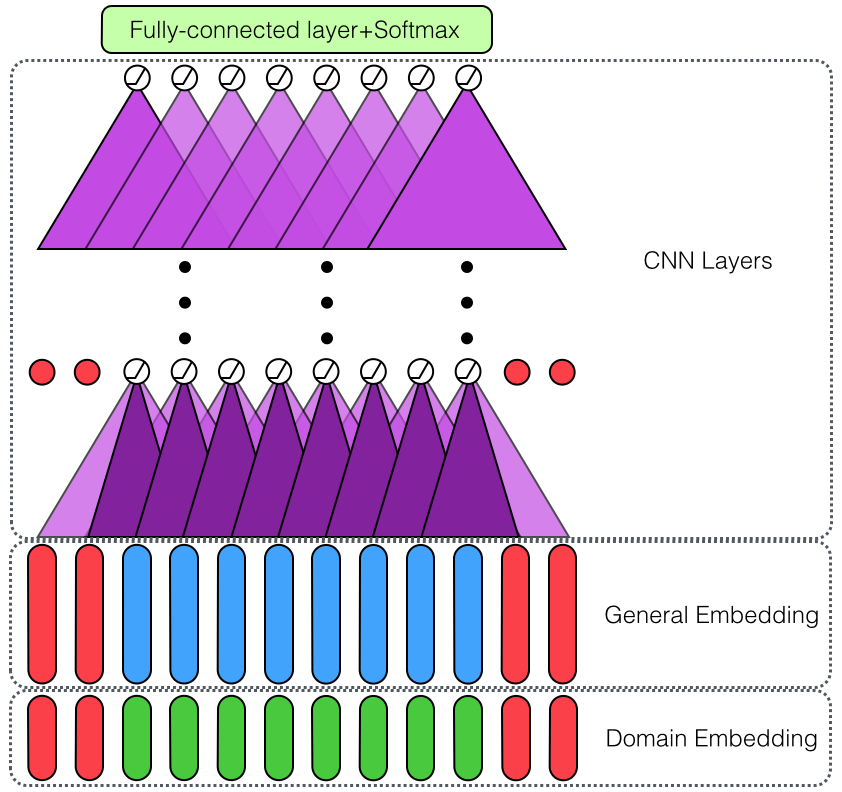
\includegraphics[width=5.in]{fig/acl18_fig.png}
    \caption{DE-CNN}
    \label{chap6:fig:fr}
\end{figure}

After leveraging the double embedding layers discussed in Chapter \ref{chap3:sec:double}, we apply CNN layers for building representations for aspect extraction.
A CNN layer is composed of 1D-convolution filters.
Each (the $r$-th) filter has a kernel size of $k=2c+1$.
Each kernel performs the following operation, followed by ReLU activation: 
%\vspace{-0.5cm}
\begin{equation}
x_{i,r}^{(l+1)}=\max\bigg(0, (\sum_{j=-c}^c w_{j,r}^{(l)} x_{i+j}^{(l)})+b_r^{(l)}\bigg),
\end{equation}
%\vspace{-0.3cm}
%\noindent
where $l$ indicates the $l$-th CNN layer. 
We apply each filter to all positions $i=1:n$.
So each filter computes the representation for the $i$-th word along with $2c$ nearby words in its context.  
Note that we force the kernel size $k$ to be an odd number and set the stride step to be 1 and further pad the left $c$ and right $c$ positions with all zeros.  
In this way, the output of each layer is well-aligned with the original input $\mathbf{x}$ for sequence labeling purposes.
For the first ($l=1$) CNN layer, we employ two different filter sizes. 
For the rest 3 CNN ($l \in \{2, 3, 4\}$) layers, we only use one filter size.
We will discuss the details of the hyper-parameters in the experiment section.
Finally, we apply a fully-connected layer with weights shared across all positions, followed by a softmax layer to classify token labels.
The output size is $|\mathcal{Y}|=3$.
We apply dropout after the embedding layer and each ReLU activation.
In contrast to common practice in computer vision, we do not apply any max-pooling operation.
This is because sequence labeling needs good position-wise representations.
But the max-pooling operation mixed representations from different positions.

We further conduct BERT model for aspect extraction. We omit the details of BERT for aspect extraction as it is already discussed in Chapter \ref{chap4:context}.

\textbf{Experiments}

\begin{table}
    \label{tab:dataset} 
    \centering
    \scalebox{0.8}{
        \begin{tabular}{c|c|c}
        \hline
            {\bf Description}  &{\bf Training }        &{\bf Testing }  \\
                               &{\bf \#S./\#A.} &{\bf \#S./\#A.}  \\\hline
            SemEval-14 Laptop  &3045/2358              &800/654\\\hline
            SemEval-16 Restaurant&2000/1743            &676/622\\\hline
        \end{tabular}
    }
    \caption{Dataset for AE}
\end{table}

Following the experiments of a recent aspect extraction paper \cite{li2017deep},
we conduct experiments on two popular datasets from SemEval \cite{pontiki2014SemEval,pontiki2016semeval}, as in Table \ref{tab:dataset}. 
Specifically, the first dataset is from the \textit{laptop} domain of SemEval-2014 Task 4.
The second dataset is from the \textit{restaurant} domain of SemEval-2016 Task 5.
These two datasets consist of review sentences with aspect terms labeled as spans of characters.
We use NLTK\footnote{\url{http://www.nltk.org/} } as the tokenizer. 

For the general-purpose embeddings, we use the glove.840B.300d embeddings \cite{pennington2014glove}, which are pre-trained from a corpus of 840 billion tokens that cover almost all web pages. These embeddings have 300 dimensions.
For domain-specific embeddings, we collect a laptop review corpus and a restaurant review corpus and use fastText \cite{bojanowski2016enriching} to train domain embeddings.  
The laptop review corpus contains all laptop reviews from the Amazon Review Dataset \cite{he2016ups}.
The restaurant review corpus is from the Yelp Review Dataset Challenge \footnote{\url{https://www.yelp.com/dataset/challenge} }.
We only use reviews from restaurant categories that the second dataset is selected from \footnote{\url{http://www.cs.cmu.edu/~mehrbod/RR/Cuisines.wht} }.
We set the embedding dimensions to 100 and the number of iterations to 30 (for a small embedding corpus, embeddings tend to be under-fitted), and keep the rest hyper-parameters as the defaults in fastText.
We further use fastText to compose out-of-vocabulary word embeddings via subword N-gram embeddings.

\textbf{Baseline Methods for DE-CNN}\\
We perform a comparison of DE-CNN with three groups of baselines using the standard evaluation of the datasets\footnote{\url{http://alt.qcri.org/semeval2014/task4}} \footnote{\url{http://alt.qcri.org/semeval2016/task5}}.
The results of the first two groups are copied from \cite{li2017deep}.
The first group uses single-task approaches.

\textbf{CRF} is conditional random fields with basic features\footnote{\url{http://sklearn-crfsuite.readthedocs.io/en/latest/tutorial.html} } and GloVe word embedding\cite{pennington2014glove}.

\textbf{IHS\_RD} \cite{chernyshevich2014ihs} and \textbf{NLANGP} \cite{toh2016nlangp} are best systems in the original challenges \cite{pontiki2014SemEval,pontiki2016semeval}.

\textbf{WDEmb} \cite{yin2016unsupervised} enhanced CRF with word embeddings, linear context embeddings and dependency path embeddings as input.

\textbf{LSTM} \cite{liu2015fine,li2017deep} is a vanilla BiLSTM.

\textbf{BiLSTM-CNN-CRF} \cite{Reimers:2017:EMNLP} is the state-of-the-art from the Named Entity Recogntion (NER) community. We use this baseline\footnote{\url{https://github.com/UKPLab/emnlp2017-bilstm-cnn-crf} } to demonstrate that a NER model may need further adaptation for aspect extraction.

The second group uses multi-task learning and also take advantage of gold-standard opinion terms/sentiment lexicon.

\textbf{RNCRF} \cite{wang2016recursive} is a joint model. It uses dependency trees for a recursive neural network. Then a layer of CRF is applied for aspect and opinion terms co-extraction. 
Besides opinion annotations, it also uses handcrafted features.

\textbf{CMLA} \cite{wang2017coupled} is a stacked network with coupled-attention. Note that it performs aspect and opinion terms co-extraction. It uses gold-standard opinion labels in the training data.

\textbf{MIN} \cite{li2017deep} is a multi-task learning framework that has (1) two LSTMs for jointly extraction of aspects and opinions, and (2) a third LSTM for discriminating sentimental and non-sentimental sentences. 
Note that this method uses a sentiment lexicon and dependency rules of high precision. 

The third group is the variations of DE-CNN.

\textbf{GloVe-CNN} only uses glove.840B.300d to show that domain embeddings are important. 

\textbf{Domain-CNN} does not use the general embeddings to show that domain embeddings alone are not good enough as the domain corpus is limited for training good general word embeddings.

\textbf{MaxPool-DE-CNN} adds max-pooling in the last CNN layer. We use this baseline to show that the max-pooling operation used in the traditional CNN architecture is harmful to sequence labeling.

\textbf{DE-OOD-CNN} replaces the domain embeddings with out-of-domain embeddings to show that a large out-of-domain corpus is not a good replacement for a small in-domain corpus for domain embeddings.
We use all \textit{electronics} reviews as the out-of-domain corpus for the \textit{laptop} and all the Yelp reviews for \textit{restaurant}.

\textbf{DE-Google-CNN} replaces the glove embeddings with GoogleNews embeddings\footnote{\url{https://code.google.com/archive/p/word2vec/} }, which are pre-trained from a smaller corpus (100 billion tokens). We use this baseline to demonstrate those general embeddings that are pre-trained from a larger corpus performs better.

\textbf{DE-CNN-CRF} replaces the softmax activation with a CRF layer\footnote{\url{https://github.com/allenai/allennlp}}. We use this baseline to demonstrate that CRF may not further improve the challenging performance of aspect extraction.

\textbf{Hyper-parameters of DE-CNN}

We hold out 150 training examples as validation data to decide the hyper-parameters.
The first CNN layer has 128 filters with kernel sizes $k=3$ (where $c=1$ is the number of words on the left (or right) context) and 128 filters with kernel sizes $k=5$ ($c=2$).
The rest 3 CNN layers have 256 filters with kernel sizes $k=5$ ($c=2$) per layer.
The dropout rate is 0.55 and the learning rate of Adam optimizer \cite{kingma2014adam} is 0.0001 because CNN training tends to be unstable.

\begin{table}
    \label{chap6:tab:result} 
    \centering
    \scalebox{0.85}{
        \begin{tabular}{c||c|c}
        \hline
        {\bf Model} &{\bf Laptop }  &{\bf Restaurant }  \\\hline
        CRF         &74.01      &69.56  \\
        IHS\_RD     &74.55      &-      \\
        NLANGP      &-          &72.34  \\
        WDEmb       &75.16      &-      \\
        LSTM        &75.25      &71.26  \\
        BiLSTM-CNN-CRF &77.8 & 72.5\\
        \hline
        RNCRF       &78.42 &-      \\
        CMLA        &77.80      &-      \\
        MIN         &77.58      &73.44  \\
        \hline
        \hline
        GloVe-CNN & 77.67 & 72.08\\
        Domain-CNN & 78.12 & 71.75\\
        MaxPool-DE-CNN & 77.45 & 71.12\\
        DE-LSTM & 78.73 & 72.94 \\
        DE-OOD-CNN & 80.21 & 74.2 \\
        DE-Google-CNN & 78.8 & 72.1 \\
        DE-CNN-CRF & 80.8 & 74.1 \\
        DE-CNN &\textbf{81.59} &\textbf{74.37} \\
        \hline
        \end{tabular}
    }
    \caption{F$_1$ score for AE}
\end{table}

\textbf{Results and Analysis of DE-CNN}

Table \ref{chap6:tab:result} shows that DE-CNN performs the best. 
The double embedding mechanism improves the performance and in-domain embeddings are important. 
We can see that using general embeddings (GloVe-CNN) or domain embeddings (Domain-CNN) alone gives an inferior performance. 
We further notice that the performance on \textit{Laptops} and \textit{Restaurant} domains are quite different. 
\textit{Laptops} has many domain-specific aspects, such as ``adapter''. 
So the domain embeddings for \textit{Laptops} are better than the general embeddings. 
The \textit{Restaurant} domain has many very general aspects like ``staff'', ``service'' that do not deviate much from their general meanings. 
So general embeddings are not bad. 
Max pooling is a bad operation as indicated by MaxPool-DE-CNN since the max pooling operation loses word positions.
DE-OOD-CNN's performance is poor, indicating that making the training corpus of domain embeddings to be exactly in-domain is important.
DE-Google-CNN uses a much smaller training corpus for general embeddings, leading to poorer performance than that of DE-CNN.
Surprisingly, we notice that the CRF layer (DE-CNN-CRF) does not help.
The CRF layer can improve 1-2\% when the laptop's performance is about 75\%.
But it doesn't contribute much when the laptop's performance is above 80\%. 
CRF is good at modeling label dependences (e.g., label $I$ must be after $B$), but many aspects are just single words and the major types of errors (mentioned later) do not fall in what CRF can solve.
Note that we did not explore the hyperparameters of DE-CNN-CRF. This is because training the CRF layer is extremely slow. 

One important baseline is BiLSTM-CNN-CRF, which is markedly worse than our method. 
We believe the reason is that this baseline leverages dependency-based embeddings\cite{levy2014dependency}, 
which could be very important for NER.
NER models may require further adaptations (e.g., domain embeddings) for opinion texts. 

DE-CNN has two major types of errors.
One type comes from inconsistent labeling (e.g., for the restaurant data, the same aspect is sometimes labeled and sometimes not). 
Another major type of error comes from unseen aspects in test data that require the semantics of the conjunction word ``and'' to extract. For example, if A is an aspect and when ``A and B'' appears, B should also be extracted but not.
We leave this to future work.

We further conduct experiments for the results of DE-CNN with language model (BERT) based methods.

\textbf{Hyper-parameters of BERT}
\label{chap6:sec:hyp}

We adopt $\textbf{BERT}_\textbf{BASE}$ (uncased) as the basis for all experiments\footnote{We expect $\textbf{BERT}_\textbf{LARGE}$ to have better performance but leave that to future work due to limited computational power.}.~Since post-training may take a large footprint on GPU memory (as BERT pre-training), we leverage FP16 computation\footnote{\url{https://docs.nvidia.com/deeplearning/sdk/mixed-precision-training/index.html}} to reduce the size of both the model and hidden representations of data.~We set a static loss scale of 2 in FP16, which can avoid any over/under-flow of floating-point computation.
The maximum length of post-training is set to 320 with a batch size of 16 for each type of knowledge. The number of sub-batch $u$ is set to 2, which is good enough to store each sub-batch iteration into a GPU memory of 11G. We use Adam optimizer and set the learning rate to be 3e-5.
We train 70,000 steps for the laptop domain and 140,000 steps for the restaurant domain, which roughly have one pass over the pre-processed data on the respective domain.

\textbf{Baseline Methods for BERT}

\textbf{BERT} is the model of the original BERT. We use this baseline to show that BERT's pre-trained weights alone have limited performance gains on review-based tasks.\\
\textbf{BERT-DK} post-trains BERT's weights only on domain knowledge (reviews) and fine-tunes on the 3 end tasks.\\
\textbf{BERT-MRC} post-trains BERT's weights on SQuAD 1.1 and then fine-tunes on the 3 end tasks.\\
\textbf{BERT-PT} (proposed method) post-trains BERT's weights using the joint post-training algorithm in Chapter \ref{chap4:sec:post-training} and then fine-tunes on the 3 end tasks.

\textbf{Results of BERT}

\begin{table}[H]
    \centering
    \scalebox{0.9}{
        \begin{tabular}{l||c|c}
        \hline
        {\bf Domain} & {\bf Laptop} & {\bf Rest.} \\
        \hline
        {\bf Methods} & {\bf F1 } & {\bf F1 } \\
        \hline
        \begin{tabular}{@{}l@{}}DE-CNN\cite{xu_acl2018}\end{tabular} & 81.59 & 74.37 \\
        \hline
        BERT  & 79.28 & 74.1 \\
        BERT-DK & 83.55 & 77.02 \\
        BERT-MRC & 81.06 & 74.21 \\
        BERT-PT & \textbf{84.26} & \textbf{77.97} \\
        \hline
        \end{tabular}
    }
    \caption{BERT for AE in F1.}
\label{chap6:tbl:result_ae}
\vspace{-5mm}
\end{table}

we found that a great performance boost comes mostly from domain knowledge post-training, which indicates that contextualized representations of domain knowledge are very important for AE. BERT-MRC has almost no improvement in restaurant, which indicates Wikipedia may not know aspects of restaurant.
We suspect that the improvements on laptop come from the fact that many answer spans in SQuAD are noun terms, which bear a closer relationship with laptop aspects.
Errors mostly come from annotation inconsistency and boundaries of aspects (e.g., apple OS is predicted as OS). Restaurant suffers from rare aspects like the names of dishes.

%\textbf{Conclusion}\\
%We propose a CNN-based aspect extraction model with a double embeddings mechanism without extra supervision.
%Experimental results demonstrated that the proposed method outperforms state-of-the-art methods with a large margin.

\subsection{-- Aspect Sentiment Classification}

As a downstream task of aspect extraction, \underline{A}spect-based \underline{s}entiment \underline{c}lassification (ASC) is to find the sentiment for an aspect appear in an opinion text.
In this subsection, we focus on two (2) improvements of ASC: (1) using pre-trained / post-trained BERT for ASC; (2) improving the post-trained BERT with the technique of hard example learning.
Hard examples are one challenge for ASC because of its datasets that are typically rare but very important for learning aspect-level sentiment (e.g., sentences with different polarities for different aspects).

\textbf{Hard Examples Learning for Aspect Sentiment Classification}

Hard examples play a non-neglectable role in many machine learning applications.
Many datasets contain a certain number of rare examples that are hard to learn, as can be found in imbalance issues or fairness issues in machine learning \footnote{\url{https://venturebeat.com/2019/01/24/amazon-rekognition-bias-mit/}}.
On one hand, the reason is from data collection that can easily and unintentionally bias a dataset.
It is very hard, if not impossible, for humans to provide an ideal dataset to a machine learning model.
As in the object detection problem \cite{shrivastava2016training,lin2017focal} in computer vision, it can easily come up with long-tailed hard examples, given it is almost impossible to manually balance objects appear in one image.
On the other hand, it is important for machine learning algorithms to avoid such issues. 

\underline{A}spect-based \underline{s}entiment \underline{c}lassification (ASC) is an important task in detecting the opinion expressed about an aspect (or an opinion target)~\cite{hu2004mining,liu2015sentiment}.
% Although sentiment classification at the document-level (or long text) can be done quite accurately, ASC is still considered as a very challenging task. 
%It not only requires fine-grained annotation of aspects and their associated opinions, but also more sophisticated classification methods.
%Unlike document-level sentiment classification where opinion terms appear frequently in a document, so it is easier to detect the overall sentiment/opinion of the document \cite{pang2002thumbs,liu2015sentiment}, detecting aspect-level sentiments in short text (e.g., a sentence) requires more accurate understanding of very fine-grained opinion expressions and also correct association of them with each opinion target (or aspect).
%For example, in ``The last thing I would buy is a windows laptop.'', there is no explicit opinion word and the expression ``The last thing I would buy'' indicating a negative opinion on ``windows laptop''. Detecting such opinion requires accurate understanding over a wide range of expressions and domain knowledge.
%For example, in ``The last thing I would buy is a windows laptop.'', there is no explicit opinion word and the expression ``The last thing I would buy'' indicating a negative opinion on ``windows laptop''. Detecting such opinion requires accurate understanding over a wide range of expressions and domain knowledge.
However, ASC also suffers from the difficulty of learning from hard examples.
For example, ``The screen is good but not the battery'' requires to detect two fine-grained and \textit{contrastive opinions} within the same sentence: a positive opinion towards ``screen'' and a negative opinion towards ``battery''.
We call this type of sentence \textbf{contrastive sentence} and \cite{jiang-etal-2019-challenge} found that such sentences are rare but hard to learn from existing ASC datasets. But these sentences are extremely important because, without them, the task of ASC turns into detecting sentence-level sentiment without the need to know the referred aspects. 
%We found that existing ASC models have great difficulty to correctly classify such contrastive opinions in their sentences. 
%As a result, obviously, successfully detecting an easy one cannot help with the detection of the other.

%\begin{table}
%    \centering
%    \scalebox{0.7}{
%        \begin{tabular}{l|c|c}
%            \hline
%            Review Sentence & Sent.-level & Asp.-level \\
%            \hline
%            The screen is good. & pos & screen: pos \\
%            \hline
%            The screen is good and also the battery. & pos & screen: pos \\
%            & & battery: pos \\
%            \hline
%            The screen is good but not the battery. & contrastive & screen: pos\\
%             &  & battery: neg\\
%            \hline
%        \end{tabular}
%    }
%    \caption{A few sentences for ASC with both sentence-level(sent.-level) polarity and aspect-level(asp.-level) polarity: the first two sentences can leverage sentence-level polarity to answer aspect-level polarity correctly but not for the last (contrastive) sentence.}
%    \label{tbl:ex_failure}
%\end{table}

%Deep supervised ASC approaches typically model ASC as a memory network~\cite{weston2014memory,sukhbaatar2015end,tang2016aspect}. Given two inputs: a sentence $x$ and an aspect term $a$ appearing in $x$, build a model $p_\theta(\hat{y}|a, x)$, where $\hat{y} \in \{\textit{pos}, \textit{neg}, \textit{neutral}\}$ is the opinion (or sentiment) about $a$.
%From the perspective of classification, this formulation is essentially a pair-wise classification task that takes a pair of inputs $(x_j, x_k)$ and predicts the class $p_\theta(\hat{y}|x_j, x_k)$. 
%as can be found in tasks such as natural language inference \cite{}, recommender system \cite{}, information retrieval \cite{}, question answering \cite{}, face recognition \cite{}, few-shot learning \cite{}, open-world learning \cite{}, etc.
%One challenge of pair-wise classification is the quadratic space of combinations introduced by the two inputs.
%This requires a huge number of critical training examples to inform the model of what the learning task is and what kinds of interactions between the two inputs are necessary for that task.
%As such, researchers propose to leverage negative sampling to obtain free negative examples and utilize more efficient (negative) examples with the hope to alleviate the requirement on the number of training examples. For example, in face recognition, \cite{} leverages \emph{close-by} face from another person as a negative example rather than using a randomly drawn negative example that is easy-to-learn and almost useless for building a high-quality model.

%For ASC, we discovered that the available datasets may not provide such rich interactions for effective supervision. 
%In fact, we observed that lacking of sentences with contrastive opinions (we call it \textbf{contrastive sentence} for brevity) can make an ASC classifier downgrading to a \underline{s}entence-level \underline{s}entiment \underline{c}lassifier (SSC), as intuitively explained in Table \ref{tbl:ex_failure}.
%By ``contrastive'', we mean two or more different opinions are associated with different aspects appearing in the same sentence.
%After all, when showing training examples with only sentences of one or more aspects with the same opinion (or polarity), the pair-wise model (or humans) can totally ignore the aspect part $a$ and only use the sentence $x$ to classify the aspect-level opinion correctly with an overall sentence-level opinion.
%Contrastive sentences are crucial for ASC, but they are infrequent, as we will see in the Dataset Analysis section.
%As a result, contrastive sentences are largely ignored in training and further weakly evaluated in the testing. 
%This results in the failure of the current ASC models incorrectly classifying contrastive opinions, as shown in the Experiments section.
% It is quite challenging for humans to discover the flaw because the evaluation results of ASC could be close to those of sentence-level classification and to understand the behavior of a trained deep learning model.

%Although in special cases humans can manually assign higher weights to rare examples contributing to the total loss (as in class imbalance problems where the human user knows the rare classes), in general, it is almost impossible for humans to discover all rare (or hard) examples from the vast input space and manually adjust their weights.
%In this paper, instead of asking humans to manually adjust the weights in the total loss, we develop a general scheme that can automatically detect those rare or hard examples and adjust their weights adaptively during the training process. Note that we are not dealing with the rare classes in the traditional class imbalance problem, but rare or hard examples in any class. 

Instead of manually addressing this issue from data collection, we focus on algorithms that automatically learn from such hard examples. 
%We propose to apply a weight to each training example, representing the importance of such an example during training.
We propose a simple training algorithm called \underline{a}daptive \underline{r}e-\underline{w}eighting (ARW), which dynamically keeps focusing on hard examples.
Since other types of hard examples are hard to identify, we thus use contrastive sentences as the proxy to evaluate ASC on hard examples.
We experimentally show that models trained with ARW significantly improve contrastive sentences, while still keep competitive or even better performance on the full set of test examples.
%The proposed training algorithm is potentially applicable to any ASC model or DL model that may have biased training data or rare but crucial examples.
%The main contribution is 2-fold: 
% \begin{itemize}
%\item 
%(1) It discovers the issue of ASC that plagues existing methods, which are clearly manifested in contrastive sentences. Such sentences are essential for the ASC task but are largely ignored.
%\item 
%(2) It proposes a re-weighting solution that resolves the issue and improves the performance on both contrastive sentences and the full set of testing examples.
% \end{itemize}
% This paper is organized as follows:
% In the next section, we first analyze the training/testing examples of a typical ASC dataset on contrastive sentences.
% Then we propose the ARW training scheme.
% In experiments, we first evaluate several state-of-the-art ASC classifiers to show their poor performance on contrastive sentences.
% Then we evaluate a wide spectrum of weighting functions and the proposed method.
% Lastly, we discuss works related to this paper and draw our conclusions.
%Then we propose several ablation studies on existing ASC baselines to test their performance beyond a simpler sentence-level sentiment classifier.
%Later, we discuss potential solutions to this issue.

\textbf{Related Work}

%The rare instance problem can be regarded as an imbalanced data problem in machine learning in general. Most existing studies in machine learning on imbalanced data focus on imbalanced classes or skewed class distributions, e.g., some classes with very few examples  \cite{huang2016learning,buda2018systematic,tantithamthavorn2018impact,johnson2019survey}. 
Hard example mining is mostly studied in object detection\cite{shrivastava2016training,lin2017focal}, which aims to detect long-tailed and imbalanced classes of sub-regions in one image.
In \cite{lin2017focal}, a loss-based weighting is proposed to adjust weights without explicitly re-balance the complex class distribution. 

Aspect sentiment classification (ASC) \cite{hu2004mining} is an essential task in aspect-based sentiment analysis \cite{pang2002thumbs,liu2015sentiment}. Aspect-based sentiment is different from document or sentence-level sentiment classification (SSC) \cite{pang2002thumbs,kim2014convolutional,he2011self,he2011automatically} as it focuses on fine-grained opinion on each specific aspect. It is either studied as a single task or a joint learning task together with aspect extraction \cite{wang2017coupled,li2017deep,li2018unified}. The problem has been widely dealt with using neural networks \cite{dong2014adaptive,nguyen-shirai-2015-phrasernn,li2018transformation}.
ASC is also studied in transfer learning or domain adaptation, such as leveraging large-scale corpora that are unlabeled or weakly labeled (e.g., using an overall rating of a review as the label) \cite{xu2019bert,he-EtAl:2018} and transferring from other tasks/domains \cite{li2018exploiting,wang2018lifelong,wang2018target}. 
Our re-weighting method is related to AdaBoost~\cite{freund1997decision}, which is a well-known ensemble algorithm that makes predictions collectively via a sequence of weak classifiers. 
Our work is different as we don’t build a sequence of classifiers like AdaBoost but only one classifier. Neither is our model an ensemble model. Our weight updating is also different from AdaBoost as we do it in each epoch of training.
We aim to improve the training process of a deep learning model by adaptively discovering incorrect examples (which cover contrastive sentences) and give them higher weights to focus on for subsequent training process. 
We also notice that AdaBoost is not frequently used in deep learning~\cite{schwenk2000boosting,mosca2017deep} probably due to the complexity of deep learning models that are not weak learners.
%Contrastive opinions are studied as a topic modeling problem in \cite{ibeke-etal-2017-extracting} to discover contrastive opinions on the same opinion target from different holders, as in discussions. However, to the best of our knowledge, existing approaches and evaluations do not focus on contrastive sentences in aspect-based sentiment classification that having opposite opinions on different aspects from the same opinion holder. But those sentences or opinions truly reveal the capability of ASC models. 

 % It is very hard, if not impossible, to manually discover and re-balance all imbalances from the input space.
 % (I removed this part as we are not dealing with the drift of testing from training, which is another area of machine learning research and we don't want to mention that as there is a large body of work on that too. We did not mention anything about data collection bias. ASC case is not due to data collection bias.) The existing biases during data collection are unavoidable in general because of the mismatch between the distribution of data during collection and the distribution of data on testing (or inferencing). On one side, the data collection is driven by cost so biases can easily be introduced into the data; on the other side, the distribution for testing keeps changing at different timestamps or being consumed by different people\footnote{https://www.vox.com/the-goods/2019/1/28/18201204/amazon-facial-recognition-dark-skinned-women-mit-study}.  

\textbf{Adaptive Re-Weighting Algorithm}
\label{sec:arw}

%In this section, we first describe the motivation for developing a new training scheme instead of following the canonical training process. 
%Then we describe the general idea of designing the \underline{a}daptive \underline{r}e-\underline{w}eighting (ARW) scheme and the detailed scheme afterward. %After that, a general property of ARW is also presented.

%\subsection{Motivation}
%Given that the examples from contrastive sentences are rare, the first question that one may ask is how a deep learning model learns from those rare examples during the existing training process.

%Intuitively, in the beginning, the losses from the majority examples dominate the total loss, and they determine the direction of parameter updates based on their gradients. 
%So the losses from majority examples can be smaller in the next few iterations. 
%At a later stage, although the loss from a rare example can be larger than the one from a majority example, the rare example still may not have enough contribution to the total loss as the loss in each batch is averaged among all examples, although the losses from the majority examples are smaller now.
%Also, as the rare examples can be rather diverse, it is unlikely that a similar rare example can later appear in another batch to have a similar impact.
%In the worst case, it is possible that the rare examples' losses are taken care of when the optimizer starts to overfit the minor details in the majority examples. When the validation process kicks in for early stopping, which aims to avoid overfitting, it may stop training the model before rare examples are really optimized well.
%To demonstrate our observation, we show how many incorrectly classified training examples are from contrastive sentences in experiments.
% Thus, deep learning models tend to learn rare examples at the later stage of training \cite{gao2016sample}.
The hardness of an example is highly associated with its rareness in a dataset because those rare examples cannot help each other in learning.
As an example, contrastive sentences are rare in ASC datasets (see Experiment).
Existing research showed that rare and noisy examples are seldom optimized at the early stage of training (e.g., a few epochs)~\cite{gao2016sample}. 
This is in contrast to its importance as discussed in the introduction.
As a result, examples should not be treated equally as the mean of example losses as in most training.
Given this unwanted behavior of optimization, a natural idea is to detect them and then increase their contribution to the total loss during training.
%Atsr asuch, rare examples are approximately equivalent to hard-to-train (we use \emph{hard} for brevity) examples in general. And, it is possible for the model to detect such hard examples at the early stage automatically.
%As long as those examples' losses are increased, those rare/hard examples can be optimized better earlier.
%One natural solution to increase those losses is to give higher weights to those examples from contrastive sentences that are not optimized well.
 % is the weighted sum of losses of examples (within a batch).
%This process of adjusting example weights could be dynamic in nature because a used-to-be easy example can be an incorrect one later and vice versa.
%For example, in ``The screen is good but not the battery.'', increasing the loss for aspect ``battery'' can make the ``screen'' incorrect later, leading to increase the loss for ``screen'' later.
%Further, note that although the model can easily access contrastive sentences based on the polarity labels during preprocessing/training, the model has no access to which example is from a contrastive sentence during validation or testing. Tackling those sentences must be automatically done during training.

%Example (or instance) (re-)weighting is also leveraged in transfer learning and domain adaptation \cite{jiang-zhai-2007-instance,foster2010discriminative,xia2013instance,wang2017instance} and sentiment analysis \cite{pappas2014explaining}, but the purpose of weighting and weighting methods are entirely different. Re-weighting is commonly used to deal with noises in the training data as well. However, its focus is to weight down possible noisy training examples/instances~\cite{rebbapragada2007class}. It is not used to improve the hard but critical examples during training like what we do.

\begin{algorithm}[!pt]
    \LinesNumbered
    \DontPrintSemicolon
    \caption{ARW Algorithm}
    %\underline{A}daptive \underline{R}e-\underline{w}eighting
    \label{alg:arw}
    \SetKwInOut{Input}{Input} 
    \SetKwInOut{Output}{Output} 
    %\SetKwRepeat{Do}{do}{while}
    \Input{$\mathcal{D}_{\text{tr}}$: training set with $n$ examples; \\$e$: maximum number of epochs.} %\\$\mathcal{D}_{\text{val}}$: validation set.}
    \Output{$p_\theta(\hat{y}|\cdot, \cdot)$: a trained model.}

    \BlankLine

%        all_y_preds=evalutate_on_train(model, eval_dataloader)
%        incorrect = (all_y_preds != all_label_ids.numpy() )
%        estimator_error = np.average(incorrect, weights=all_sample_weights.numpy(), axis=0)
%        estimator_weight = np.log((1. - estimator_error) / estimator_error)
%        scale=np.exp(estimator_weight * incorrect)
%        all_sample_weights.mul_(torch.from_numpy(scale).float() )

%    $\mathcal{T} \gets \{\}$ \;
    $w_{1:n} \gets \frac{1}{n} $ \;
    %\tcp*{Initialize all example weights uniformly.}
    \For{$\text{epoch} \in \{1, \dots, e\}$}{ %\tcp*{Pass through the training data epoch-by-epoch.} }{
        \For{$(a^b, x^b, y^b, w^b) \in \text{Batchify}(\mathcal{D}_{\text{tr}}, w_{1:n})$}{ %\tcp*{Retrieve one randomly sampled batch.}}{
            $l^b \gets \text{CrossEntropy}(p_\theta(\hat{y}^b|a^b, x^b), y^b)$ \; %\tcp*{Compute example-wise loss.}
            $L^b \gets \frac{\sum(w^b \cdot l^b)} {\sum w^b}$ \; %\tcp*{Re-normalize weighted loss and compute total loss.}
            $\text{BackProp\&ParamUpdate}(L, M)$ \;   %\tcp*{Back propagation and parameter updates.}
        }
        $\hat{y}_{1:n}\gets \argmax p_\theta(\hat{y}_{1:n}|a_{1:n},x_{1:n})$ \; %\tcp*{Compute current prediction.}
        $r \gets \frac{\sum_{i=1}^{n}(w_i\mathbb{I}[y_{i}\neq \hat{y}_{i}])}{\sum_{i=1}^n w_i}$ \; %\tcp*{Compute weighted error rate.} \wedge \text{Contra}(x_i)
        $\alpha \gets \log(\frac{(1-r)+\epsilon}{r-\epsilon})$ \; %\tcp*{Compute the log correct-incorrect ratio.}
        % for loop
        $w_{1:n} \gets w_{1:n} \exp(\alpha \mathbb{I}[y_{1:n} \neq \hat{y}_{1:n} ])$ % \wedge \text{Contra}(x_{1:n}) ])$ %\tcp*{Adjust weights of incorrect examples.}
        
    %        $x \gets \texttt{[CLS]} $ \;
    %        $h \gets \text{RandInteger}([0, h_{\text{max}}]) $ \;
    %        \For{$1 \to h$}{
    %            $q'', a'' \gets \text{RandSelect}(\mathcal{Q}\backslash(q', a'))$ \;
    %            $ x \gets x \oplus \texttt{[Q]} \oplus q'' \oplus \texttt{[A]} \oplus a'' $\;
    %        }
    %        $ x \gets x \oplus \texttt{[Q]} \oplus q' \texttt{[SEP]} $ \;
    %        $ r_{1:m} \gets \text{RandSelect}(\mathcal{R}) $ \;
    %        \If{$\text{RandFloat}([0.0, 1.0]) > 0.5$ }{
    %            $(\_, a) \gets \text{RandSelect}(\mathcal{Q}\backslash(q', a') ) $ \;
    %            $(u, v) \gets (1, 1)$ \;
    %        }
    %        \Else{$a \gets a'$ \;
    %            $(u, v) \gets (|x|, |x|+|a|) $ \;
    %        }
    %        $ l \gets \text{RandInteger}([0, u]) $ \;
    %        $ d_{1:n} \gets r_{0:l} \oplus a \oplus r_{l+1:u} $ \;
    %        \If{$u>1$ }{
    %            $ (u, v) \gets (u+|r_{0:l}|, v+|r_{0:l}|) $
    %        }
    %        $x \gets x \oplus d_{1:n} \oplus \texttt{[SEP]}$ \;
    %        $\mathcal{T} \gets \mathcal{T} + (x, (u, v) )$ \;
    }
\end{algorithm}

Since training in supervised learning has access to ground-truth labels, detecting hard examples naturally means to find examples the current model cannot classify correctly.
Assuming we have $n$ training examples.
Let incorrect (hard) examples to be those with $y_{i}\neq \hat{y}_{i}$ for $i \in [1, n]$, where $\hat{y}_{i}$ is the prediction of the $i$-th training example from the current model and $y_{i}$ is the ground-truth label.
Then we associate each example a weight, which decides how much this example contributes to the total loss (e.g., in a batch of optimization).
We let $w_{1:n}$ denote the weights associated with $n$ training examples and the total loss of $L$ is computed as the weighted sum of the training examples. 
%So an example with a higher weight is more likely to contribute more to $L$.
As deep learning models are typically trained on a batch-by-batch basis, we define the total loss $L^b$ as the loss from a batch.
Let $l^b$ be the example-wise losses for examples within a batch. 
Since a batch is randomly drawn from the training set, we re-normalize the weights $w^b$ for examples in that batch $L^b=\frac{\sum(w^b \cdot l^b)} {\sum w^b}$ to avoid fluctuation caused by randomly drawing examples with weights of different magnitudes.

Given the dynamics of a training process, we aim to design an adaptive weighting function that keeps adjusting the weights.
This is because a used-to-be hard example can later be an easy example and vice-versa.
%We assume the training algorithm has no knowledge about which examples are hard or not at the beginning. 
At the beginning, we assume an uniform distribution of weights across all training examples $w_{1:n} \gets \frac{1}{n} $.
We adjust the weights at the end of the training of each epoch because every example has been consumed once.
We define an indicator variable $\mathbb{I}[y_{i} \neq \hat{y}_{i}]$ to pick the incorrect (hard) examples and estimate the overall weighted error rate $r \in [0, 1]$ to detect whether the current model tends to make more mistakes or not. 
Note that the reason for using the weighted error rate instead of just the error rate is that the weighted error rate reflects the hardness on optimizing hard examples instead of simply example-level errors. We will detail the formula in the next subsection.
For example, when the weighted error rate is high (e.g., $>0.5$), instead of increasing the weights for incorrect examples, we probably need to reduce them so as to avoid learning too much noise.
Lastly, the weight adjustment for incorrect examples is determined by the (correct-versus-incorrect) ratio $(\frac{(1-r)+\epsilon}{r-\epsilon})$. So when this value is larger than $1$, multiply it to increase the weights; otherwise to decrease the weights.
Here we introduce a weight assignment factor $\epsilon$, which is a hyperparameter to control whether the model should favor even more weights (e.g., $\epsilon>0$) or not (e.g., $\epsilon<0$).

\textbf{ARW Algorithm}

The proposed ARW algorithm is shown in Algorithm \ref{alg:arw}.
In Line 1, it initializes the weights of all training examples uniformly.
Lines 2-12 pass through the training data epoch-by-epoch and update the example weights at the end of each epoch.
Specifically, Line 3 retrieves one randomly sampled batch of aspects $a^b$, sentences $x^b$, polarity labels $y^b$ and their (current) corresponding weights $w^b$.
Line 4 makes a forward pass on aspects and sentences $p_\theta(\hat{y}|a^b, x^b)$. Then we compute example-wise loss $l^b$ for each training example in the batch.
Line 5 computes the weighted loss and re-normalize these weights throughout the batch to get the total loss $L^b$. 
%This re-normalization ensures the scale of total loss is not affected much by re-weighting and random sampling of a batch. 
Line 6 does normal backpropagation and parameter updating as in ordinary neural networks training.
%Lines 10 to 13 are essential to the algorithm as they examine hard examples and compute new weights for them (?? we have not explained the weight assignment equations).
Line 8 gets the prediction on the training set.
Line 9 first discovers the hard examples represented by an indicator variable $\mathbb{I}[y_{i}\neq \hat{y}_{i}] $.
It then computes the weighted error rate. 
%In this way, the error does not measure example-level error (?? weird sentence) but the overall hardness of the current model's performance on the training set (not quite understandable).
Line 10 computes the log of the correct-incorrect ratio. $\alpha >0$ indicates increasing the weights and $\alpha<0$ means decreasing the weights.
Lastly, in Line 11, we only adjust the weights via the indicator variable $\mathbb{I}[y_{1:n} \neq \hat{y}_{1:n}]$ since the weights of correctly classified (easy) examples are always multiply by $1$.
As a result, Algorithm \ref{alg:arw} keeps track of the weights $w_{1:n}$ for all training examples and always focuses on adjusting weights of incorrect examples from contrastive sentences. We also perform a normal validation process after each epoch (omitted in the Algorithm \ref{alg:arw} for brevity).
%(?? how much weights are assigned to hard cases and how to compute the weights are very important, but are not described in detail)
%Given this algorithm has the same requirement as in supervised learning, it is general and can potentially be used to train any model with various biases.


%\subsubsection{Proof of Property (?? what property?)}
%One nice property of the ARW algorithm is that it intends to re-weight the total weights for hard (or incorrect) examples to (?? what is 'to the') the total weights of easy (or correct) examples (?? cannot understand this sentence). We illustrate this property via Eq. \ref{eq:eq}. Let the left side of Line 12 of Algorithm \ref{alg:arw} be $w_{1:n}'$. We simplify 
%$\mathbb{I}[y_{1:n} \neq \hat{y}_{1:n}]$ as $\mathbb{I}_\text{hard }$ and $\mathbb{I}[y_{1:n} = \hat{y}_{1:n}]$ as $\mathbb{I}_\text{easy}$.
%So $\sum w_{1:n}'\mathbb{I}_\text{hard} $ indicates the newly adjusted total weights for hard examples.

%\begin{equation}
%\label{eq:eq}
%\begin{split}
%\sum w_{1:n}'\mathbb{I}_\text{hard} = \sum w_{1:n} \exp (\alpha \mathbb{I}_\text{hard} ) \mathbb{I}_\text{hard} \\
%= (\sum w_{1:n} \mathbb{I}_\text{hard}) \exp \big(\log (\frac{\sum w_{1:n} \mathbb{I}_\text{easy} }{\sum w_{1:n} \mathbb{I}_\text{hard}} ) \big) \\
%= (\sum w_{1:n} \mathbb{I}_\text{hard}) \frac{\sum w_{1:n} \mathbb{I}_\text{easy} }{\sum w_{1:n} \mathbb{I}_\text{hard}} \\
%= \sum w_{1:n} \mathbb{I}_\text{easy} \\
%\end{split}
%\end{equation}

%From Eq. \ref{eq:eq}, we can see that the ARW algorithm essentially adjusts the total weights for hard examples to the (?? what you mean by 'to the'?) total weights of easy examples so to balance the total weights for correct and incorrect examples.

\textbf{Experiment}
\label{sec:exp}

%Our experiment consists of two parts: (1) show the failure of existing approaches and (2) demonstrate the effectiveness of the ARW scheme.
%We focus on the following research questions (RQs):\\
%\textbf{RQ1}: How is the performance of existing ASC systems on the contrastive sentences in the test data (\emph{Contrastive Test Set}) ?\\
%\textbf{RQ2}: What is the performance of an ASC model trained from data with manually assigned fixed higher weights to contrastive sentences only? \\
%\textbf{RQ3}: How is the performance of the proposed ARW system compared with the above baselines?\\
%\textbf{RQ4}: How is the performance of a loss-based weighting function (such as the famous focal loss \cite{lin2017focal}) compared to ARW?\\
%\textbf{RQ5}: How important is the term $\text{Contra}(\cdot)$ (in Lines 11 and 13), given it needs preprocessing to find which sentence is contrastive?\\
%\textbf{RQ6}: Can ARW tackle more examples from contrastive sentences before early stopping (via the validation set) ?

\textbf{Dataset}

We adopt the SemEval 2014 Task 4\footnote{http://alt.qcri.org/semeval2014/task4} datasets, which 
%to demonstrate how rare those contrastive sentences are. These datasets 
contain two domains: \emph{laptop} and \emph{restaurant}. 
The statistics are shown in \ref{chap6:tbl:asc}. In addition to the \textit{Full Testing Set}, we further form a \textit{Contrastive Test Set} to specifically test aspect-level sentiments.
The contrastive test set of laptop is augmented with extra annotated examples from Amazon laptop reviews to ensure enough testing examples. 
%We further demonstrate that the normal training on such datasets results in poor performances on contrastive sentences in experiments.

%To solve this problem, two (2) annotators are asked to follow the annotation instructions of SemEval 2014 Task 4 and annotate more contrastive sentences (to have a similar number of contrastive sentences as \emph{restaurant} in total) from Laptop reviews~\cite{he2016ups}.
%Disagreements are discussed until agreements are reached.


\begin{table}
\centering
\scalebox{0.7}{
    \begin{tabular}{l|c|c}
    \hline
    & \bf{Laptop} & \bf{Restaurant} \\
    \hline
    \bf{Training} & & \\
    \hline
    \#Sentence & 3045 & 2000 \\
    \#Aspect & 2358 & 1743 \\
    \#Positive & 987 & 2164 \\
    \#Negative & 866 & 805 \\
    \#Neutral & 460 & 633 \\
    \#Sent. /w Asp. & 1462 & 1978 \\
    \hline
    \#Contrastive Sent. & \textbf{165} & \textbf{319} \\
    \%Contrastive Sent. & \textbf{11.3\%} & \textbf{16.1\%} \\
    %\#Asp. in Sent /w mixed opinions & 455 & 940 \\
    \hline
    \bf{Full Testing Set} & & \\
    \hline
    \#Sentence & 800 & 676 \\
    \#Aspect & 654 & 622 \\
    \#Positive & 341 & 728 \\
    \#Negative & 128 & 196 \\
    \#Neutral & 169 & 196 \\
    \#Sent. /w Asp. & 411 & 600 \\
    \hline
    \#Contrastive Sent. & \textbf{38} & \textbf{80} \\
    \%Contrastive Sent. & \textbf{9.2\%} & \textbf{13.3\%} \\
    \hline
    \bf{Contrastive Test Set} & & \\
    \hline
    \#Contrastive Sent. & \textbf{78} & \textbf{80} \\
    \#Aspect & 203 & 228 \\
    \#Positive & 72 & 85 \\
    \#Negative & 71 & 60 \\
    \#Neutral & 60 & 83 \\
    \hline
    
    \hline
    \end{tabular}
}
\caption{Statistics of SemEval14 Task4 with Contrastive sentences}
% are rare. \%Contrastive Sent.: means the percentage of contrastive sentences in sentences with at least one aspect.}
%\#Sentence: number of sentences; \#Aspect: number of aspects; \#Positive, \#Negative, and \#Neutral: number of aspects with positive, negative and neutral opinions, respectively; \#Sent. /w Asp.: number of sentences with at least one aspect that is associated with one of positive, negative or neutral opinion; \#Contrastive Sent.: number of sentences with aspects associated with different opinions; \%Contrastive Sent.: percentage of contrastive sentences in sentences with at least one aspect.}
\label{chap6:tbl:asc}
\end{table}

%As shown in Table \ref{tbl:asc}, we first examine the overall statistics of these datasets.
%We decompose these statistics to get deeper insights that may lead to a failed ASC classifier. 
%We notice that although these datasets contain a moderate number of training sentences for laptop, sentences with at least one aspect (and thus has polarities of opinions) is less than 50\%, as in \emph{\#Sent. /w Asp}. 
% We examined a few examples and quickly noticed that besides opinions on aspects, \emph{Laptop} reviewers tend to talk about other issues such as specs.

%Further, as discussed in the introduction, we are particularly interested in contrastive sentences that have more than one aspect and are associated with different opinions (\textit{\#Contrastive Sent.}) for each such sentence.
%Those sentences carry critical training examples (information) for ASC because the rest of the examples have only one polarity per sentence (even with two or more aspects), where the overall sentence-level opinion can be applied to aspect-level opinion and thus effectively downgrade the task of ASC to SSC (sentence-level sentiment classification).

%We notice that contrastive sentences are rare in both training and test sets of both domains. Laptop is even more so on the shortage of contrastive sentences because of the shortage of sentences with at least one aspect.

%If we consider their percentage (\textit{\%Constrastive Sent.}), the training set of restaurant has just about \textbf{16\%} and the laptop has only about \textbf{11\%}. With the SSC-like examples dominating the training set, a machine learning model trained on such a set is susceptible to ignoring the aspect and mostly performing SSC.% (sentence sentiment classification).

%What is worse is that the test set for the \emph{laptop} domain contains only 38 contrastive sentences.
%This further poses a challenge on evaluating the ASC capability for \emph{laptop} as only contrastive sentences can evaluate the true capability of ASC. 



%The main complaint from the annotators is that finding such sentences takes a lot of time as they are infrequent.
% This indicates that human can easily make such mistakes on supervision given the existing distribution of data.
%By combining the additional contrastive sentences with those contrastive sentences from the original test set, we form a new \emph{contrastive test set}, dedicated to testing the true ASC capability of ASC classifiers. Note that there is no change to the training set for the laptop domain and no change to either the training or the test set of the restaurant domain. The final statistics of the contrastive sentence are shown in Table \ref{tbl:our}.
%To simplify our description, we refer to the original test set as the \emph{full test set}.
%Note that we DO NOT add those extra contrastive sentences into the full test set to keep the results comparable with existing approaches.
%We evaluate the failure of existing ASC classifiers on the contrastive test set in experiments and discuss our example re-weighting scheme that focuses training on rare contrastive sentences in the next section.

%\begin{table}
%\caption{Summary of SemEval14 Task4 on aspect sentiment classification. \#Sent: number of sentences; \#Asp: number of aspects; \#Pos., \#Neg., and \#Neu.: number of aspects with \underline{pos}itive, \underline{neg}ative and \underline{neu}tral polarities, respectively.}
%\centering
%\scalebox{0.8}{
%    \begin{tabular}{l|c c c c c}
%    \hline & \#Sent. & \#Asp. & \#Pos. & \#Neg. & \#Neu \\
%    \hline
%    \bf{Laptop} & & & & & \\
%    \hline
%    Training & 3045 & 2358 & 987 & 866 & 460 \\
%    Testing & 800 & 654 & 341 & 128 & 169 \\
%    \hline
%    \bf{Restaurant} & & & & & \\
%    \hline
%    Training & 2000 & 1743 & 2164 & 805 & 633 \\
%    Testing & 676 & 622 & 728 & 196 & 196 \\
%    \hline
%    \end{tabular}
%}
%\label{tbl:asc}
%\end{table}

%\section{The Proposed Adaptive Example Re-weighting Scheme}


%\textbf{datasets}

%For ASC, we use SemEval 2014 Task 4 for both laptop and restaurant as existing research frequently uses this version. We use 150 examples from the training set of all these datasets for validation.
\textbf{Results of BERT}

We first discuss the results of post-training BERT from Chapter \ref{chap4:context}. We have the following state-of-the-art baseline:\\
\textbf{MGAN} \cite{li2018exploiting} reaches the state-of-the-art ASC on SemEval 2014 task 4.
We compute both accuracy and Macro-F1 over 3 classes of polarities, where Macro-F1 is the major metric as the imbalanced classes introduce biases on accuracy.~To be consistent with existing research \cite{tang2016aspect}, examples belonging to the \textit{conflict} polarity are dropped due to a very small number of examples.

\begin{table}
    \centering
    \scalebox{0.78}{
        \begin{tabular}{l||c c|c c}
        \hline
        {\bf Domain} & {\bf Laptop} & & {\bf Rest.} & \\
        \hline
        {\bf Methods} & \bf{Acc.} & \bf{MF1} & \bf{Acc.} & \bf{MF1} \\
        \hline
        \begin{tabular}{@{}l@{}}
        MGAN \cite{li2018exploiting}\end{tabular} & 76.21 & 71.42 & 81.49 & 71.48 \\
        \hline
        BERT & 75.29 & 71.91 & 81.54 & 71.94 \\
        BERT-DK & 77.01 & 73.72 & 83.96 & 75.45 \\
        BERT-MRC & 77.19 & 74.1 & 83.17 & 74.97 \\
        BERT-PT & 78.07 & \textbf{75.08} & 84.95 & \textbf{76.96} \\
        \hline
        \end{tabular}
    }
    \caption{ASC in Accuracy and Macro-F1(MF1).}
\label{chap6:tbl:result_asc}
\vspace{-5mm}
\end{table}

ASC, we observed that large-scale annotated MRC data is very useful.
We suspect the reason is that ASC can be viewed as a special MRC problem. For example, all questions are about asking the polarity of some aspects.
MRC training data may help BERT to understand the input format of ASC given their closer input formulation.
Again, domain knowledge post-training also helps ASC.
ASC tends to have more errors as the decision boundary between the negative and neutral examples is unclear (e.g., even annotators may not sure whether the reviewer shows no opinion or slight negative opinion when mentioning an aspect).
Also, BERT-PT has the problem of dealing with one sentence with two opposite opinions (``The screen is good but not for windows.''). We believe that such training examples are rare.

Next we discuss the results of ARW.

\textbf{Baselines for ARW}
\label{chap6:sec:baselines}

%To demonstrate existing ASC systems' difficulty with contrastive sentences, we used a range of ASC baselines and tested their performance on examples from contrastive sentences (contrastive test set). 
We evaluate all baselines on both accuracy (Acc.) and macro F1 (MF1) and adopt the following baselines:
%\noindent
RAM~\cite{chen2017recurrent}\footnote{The first 4 baselines are adopted from \url{https://github.com/songyouwei/ABSA-PyTorch}.},
%This system proposes a multiple-attention mechanism to capture sentiment features separated by a long distance so that it is more robust against irrelevant information. The weighted-memory and attention mechanism not only helps avoid the labor-intensive feature engineering work but also provides a tailor-made memory for different opinion targets of a sentence.\\
AOA~\cite{huang2018aspect},
%This system introduces an attention-over-attention (AOA) neural network, which models aspects and sentences in a joint manner and explicitly captures the interaction between aspects and the sentence context.\\
MGAN~\cite{li2018exploiting},
%This method leverages the fine-grained and coarse-grained attention mechanisms to compose the MGAN framework. It also has an aspect alignment loss to depict the aspect-level interactions among aspects that have the same context.\\
TNET~\cite{li2018transformation}. 
%This system employs a CNN layer to extract salient features from the transformed word representations originated from a bi-directional RNN layer. Between the two layers, TNET has a component to generate target-specific representations of words while incorporating a mechanism for preserving the original contextual information from the RNN layer.\\
BERT-DK~\cite{xu2019bert}\footnote{\url{https://github.com/howardhsu/BERT-for-RRC-ABSA}}. 
%This is the BERT-based model \cite{devlin2018bert}. It achieved the state-of-the-art results on ASC recently. 
%Based on BERT, it first performs masked language modeling and then next sentence prediction on pre-trained BERT weights using domain (laptop or restaurant) reviews. Then it is fine-tuned using supervised ASC data.
%We choose BERT-DK because of its easy-to-understand implementation without extra supervised tasks (such as reading comprehension) and its performance.
For the last model, we further challenge it by removing the aspects from the testing examples as there is no architecture change in doing so. 
In this way, we want to test the performance of BERT-DK under a setting with no access to aspects. 
%We want to see whether its performance on the \emph{Full Test Set} is affected much or not. Note that this is not a traditional sentence-level classifier as the training process is still under ASC task. % This is effectively a sentence-level sentiment classification.  

\begin{table}
\centering
\scalebox{0.5}{
    \begin{tabular}{l|c c|c c}
    \hline
     & \bf{Laptop} & & \bf{Rest.} & \\
    \hline
    
%AOA laptop
%0.6065830721003135 0.6190703143863948
%0.42857142857142855 0.3353321274448432

%AOA restaurant
%0.6875 0.42114903610982085
%0.4298245614035088 0.3365772426829434

%MGAN laptop
%0.6206896551724138 0.5906459172798848
%0.46798029556650245 0.4338355880433239

%MGAN restaurant
%0.7214285714285714 0.595698169830283
%0.5394736842105263 0.5764384420322586

%TNET laptop
%0.6818181818181818 0.6324295523192144
%0.4975369458128079 0.4986077778110347

%TNET Restaurant
%0.7401785714285715 0.6202234956434919
%0.5657894736842105 0.5805174216041218

     & Acc. & MF1 & Acc. & MF1 \\
    \hline
    RAM\cite{chen2017recurrent} & & & & \\
    on Full Test Set & 74.49 & 71.35 & 80.23 & 70.8 \\
    on Contrastive Test Set & 41.87 & 38.65 & 52.19 & 55.19 \\     
    \hline
    AOA\cite{huang2018aspect} & & & & \\
    on Full Test Set & 74.5 & - & 81.2 & - \\
    on Contrastive Test Set & 42.86 & 33.53 & 42.98 & 33.66 \\
    \hline
    MGAN\cite{li2018exploiting} & & & & \\
    on Full Test Set & 75.39 & 72.47 & 81.25 & 71.94 \\
    on Contrastive Test Set & 46.8 & 43.38 & 53.95 & 57.64 \\
    \hline
    TNET\cite{li2018transformation} & & & & \\
    on Full Test Set & 76.54 & 71.75 & 80.69 & 71.27 \\
    on Contrastive Test Set & 49.75 & 49.86 & 56.58 & 58.05 \\
    \hline
    BERT-DK\cite{xu2019bert} & & & & \\
    on Full Test Set & 76.9 & 73.65 & 84.21 & 76.2 \\
    on Full Test Set \textbf{w/o} aspect & \underline{76.0} & \underline{73.05} & \underline{80.03} & \underline{72.95} \\
    %Trained on MultiDomain & 77.99 & 75.26 & 83.67 & 75.93 \\
    on Contrastive Test Set & 51.13 & 50.04 & 65.53 & 66.92 \\
    %Trained on MultiDomain & 51.17 & 55.61 & 64.91 & 67.19 \\
    \hline
    \hline
    BERT-DK & Acc. & MF1 & Acc. & MF1 \\
    \hline
    + Manual Re-weighting & & & & \\
    on Full Test Set & 75.41 & 71.99 & 84.36 & 76.35 \\
    on Contrastive Test Set & 53.45 & 52.76 & 68.03 & 69.51 \\
    \hline
    + Focal Loss\cite{lin2017focal} & & & & \\
    on Full Test Set & 76.33 & 73.24 & 84.57 & 76.56 \\
    on Contrastive Test Set & 51.48 & 50.43 & 66.4 & 67.14 \\
    \hline
    %+ ARW & & & & \\
    %on Full Test Set & 73.71 & 69.63 & 84.5 & 77.58 \\
    %on Contrastive Test Set & 57.29 & 56.53 & 73.99 & 74.63 \\
    %\hline
    + ARW w/ manual initial weighting & & & & \\
    on Full Test Set & 70.08 & 65.89 & 84.48 & 77.41 \\
    on Contrastive Test Set & 55.37 & 54.68 & \textbf{75.31} & \textbf{75.81} \\
    \hline
    %+ ARW \textbf{w/o} $\text{Contra}(\cdot)$ & & & & \\
    + ARW & & & & \\
    on Full Test Set & \textbf{77.23} & \textbf{73.81} & \textbf{85.35} & \textbf{78.46} \\
    on Contrastive Test Set & \textbf{61.08} & \textbf{60.34} & \textbf{71.84} & \textbf{72.66} \\
    \hline
    \end{tabular}
}
\caption{Results of ARW on ASC}
%baselines and the proposed ARW Scheme on both \emph{Full Test Set} and \emph{Contrastive Test Set}; the BERT-DK model is further tested on examples by removing aspects as in (\emph{on Full Test Set w/o aspect}).}
\label{chap6:tbl:failure}
\end{table}

\vspace{-2mm}

%\subsubsection{Baseline Result Analysis}
 % and existing evaluation is problematic on evaluate aspect-level sentiment.
% (? I edit a bit. ?? this paragraph is problematic. The drop is not slight, but quite significant, which shows that aspects are useful. Any explanation? We may not say ``downgraded to sentence-level classification.'').

%\subsection{ARW}
%The results of the above subsection justify the need for evaluating ASC on the contrastive test set and the need to improve the performance on that set. Since an ideal ASC should also be fully functional on none contrastive sentences, we still need to evaluate ARW and baselines on the full test set. In this set of experiments, we focus on ARW alone with various re-weighting schemes. %  but ARW is generally applicable to any deep learning models.
%\textbf{No Re-weighting}. This is the same as BERT-DK as ARW is built on top of it.  \\ %To ease the comparison with other baselines, we copy the numbers of BERT-DK from Table \ref{tbl:failure}. \\
%\subsubsection{Compared Methods} 
We use BERT-DK as a base model to compare the following re-weighting schemes.\\
\textbf{+Manual Re-weighting.}
%This baseline uses pre-defined weights for examples from contrastive / non-contrastive sentences.
%a natural way to balance the examples from contrastive sentences and non-contrastive sentences is to use the number of examples as weights.
This baseline first counts the number of training examples $C_c$ that are contrastive sentences and gives these examples/sentences the weight $(n-{C_c})$ and other examples the weight $C_c$, where $n$ is the total number of training examples. 
%So examples from contrastive sentences are expected to receive higher weights.
These weights are re-normalized within a batch. 
Note that we also experimented with a number of other manual weighting schemes and this method does the best. \\
%(? I dont understand this but anyway revise a lot here. ?? I don't understand this part. Identifying contrastive sentences is not hard in ASC. Defining proper weights is also an issue for ARW. I think we should not stress this manual effort unless for different data/domains different weights are needed. We just say we tried many ways of weighting and the current way performed the best.)
%Note that this baseline requires extensive efforts from humans on discovering the flaws of existing models, picking out examples from contrastive sentences and defining proper weights for those examples.\\
\textbf{+Focal Loss.} We compute weights as $(1-p)^\gamma$ \cite{lin2017focal}, where $p$ is the probability of prediction on the ground-truth label (from softmax) and $\gamma$ is a hyper-parameter. We use $\gamma = 2.0 $ from the original paper that works best for ASC, too.\\ % no assumption about humans to discover the issue of rare true examples for ASC.
%\textbf{+ARW} This is the proposed training scheme, which is intended to answer RQ3.\\ % no assumption about humans to discover the issue of rare true examples for ASC.
\textbf{+ARW.} This is the proposed training algorithm. This method discovers all incorrect examples, which include examples from the contrastive sentences set and other examples. We search $\epsilon \in \{-0.2, -0.1, -0.05, 0.0, 0.05, 0.1, 0.2\}$ and use $\epsilon = -0.05 $ for results.\\
\textbf{+ARW w/ manual initial weighting.} We further investigate the use of +Manual Re-weighting's weighting function as the initial weights and then use ARW for adaptive re-weighting.
%\begin{table}[t]
%\centering
%\scalebox{0.75}{
%    \begin{tabular}{l|c c|c c}
%    \hline
%    BERT-DK & \bf{Laptop} & & \bf{Rest.} & \\
%    \hline
%     & Acc. & F1 & Acc. & F1 \\
%    \hline
%    No Re-weighting & & & & \\ 
%    - on Full Test Set & 76.85 & 73.58 & 83.75 & 75.12 \\
%    - on Contrastive Test Set & 47.86 & 51.99 & 63.2 & 63.74 \\
%    \hline
%    Manual Re-weighting & & & & \\
%    - on Full Test Set & 75.58 & 71.97 & 84.93 & 77.45 \\
%    - on Contrastive Test Set & 51.84 & 54.99 & 69.74 & 71.33 \\
%    \hline
%    ARW & & & & \\
%    - on Full Test Set & 76.03 & 73.05 & \textbf{85.15} & \textbf{78.15} \\
%    - on Contrastive Test Set & \textbf{62.56} & \textbf{62.32} & \textbf{70.31} & 70.35 \\
%    \hline
%    \end{tabular}
%}
%\caption{Performance of baselines and ARW on ASC.}
%\label{tbl:bal_contra}
%\end{table}

\textbf{Hyper-parameters}

%(?? the writing of this part should also be careful as we said we build on top of Bert-DK) 
%We leverage the base model of BERT to be consistent with the existing paper \cite{xu_bert2019}. 
For all methods, we use Adam optimizer and set the learning rate to 3e-5. The batch size is set as 32.
To perform model selection, we hold out 150 examples from the training set as the validation set.
%We experimentally found that ARW takes longer time to converge compared with the ordinary training of a BERT-based model. 
%For the \emph{Laptop} domain, it typically converges on the 8th or 9th epoch; for the \emph{restaurant} domain it converges on the 5th or 6th epoch. 
We set the maximum epochs to 12.
Lastly, all results are averaged over 10 runs.
%\subsubsection{ARW Result Analysis}
%\begin{table}[t]
%\centering
%\scalebox{0.7}{
%    \begin{tabular}{l|c|c}
%    \hline
%    & \bf{Laptop} & \bf{Restaurant} \\
%    \hline
%    \# total examples & 2163 & 3452 \\
%    \hline
%    BERT-DK & & \\
%    \# incorrect examples & 208 & 290 \\
%    \# incorrect examples from contra. sent. & 148 & 228 \\
%    \hline
%    BERT-DK +ARW w/o $\text{Contra}(\cdot)$ & & \\
%    \# incorrect examples & 48 & 360 \\
%    \# incorrect examples from contra. sent. & \textbf{47} & \textbf{201} \\
%    \hline
%    \end{tabular}
%}
%\caption{Number of incorrectly predicted training examples (\# incorrect examples from contra. sent.) from contrastive sentences in one run of training: the training of the model is early stopped by validation set.}
%\label{tbl:pred}
%\end{table}
\textbf{Result Analysis}

From \ref{chap6:tbl:failure}, %we can see existing ASC classifiers perform poorly on the contrastive test sets. %, which contain real ASC examples only.
we can see that all existing ASC baselines have significant drops on the contrastive test set for both Accuracy (Acc.) and F1 score, indicating the hardness of this testing set.
%as most existing models reach more than 70\% on both accuracy and F1 on the full test set.
%Lastly, 
When the aspects are dropped from the input (\emph{on Full Test Set w/o aspect}), the BERT-DK ASC classifier dropped a little and still comparable to other baselines on the full test set.
%, which means 
%Since this experiment has no access to aspects but just the review sentences, %it indicates that 
%the model \textbf{DOES NOT} count on aspects much in doing aspect-level sentiment classification.
%The results are also shown in Table \ref{tbl:failure}.

\emph{BERT-DK + ARW} outperforms other baselines mostly. If we compare it with \emph{BERT-DK}, it gives nearly 10\% of improvement for laptop and 6\% for restaurant on the contrastive test set.
%Regarding the overall performance on the full test set, \emph{BERT-DK + ARW w/o $\text{Contra}(\cdot)$} has a marked improvement overall in the restaurant domain.
%When we examine the examples, the contribution is largely from neutral examples.
%Its performance on laptop is slightly better than \emph{BERT-DK}.
%One reason could be that the examples from contrastive sentences are too rare compared to annotation errors in laptop. So the model learns some annotation errors.
%Overall, these numbers indicate that \emph{BERT-DK + ARW w/o $\text{Contra}(\cdot)$} still functions well overall based on the traditional evaluation of ASC, but significantly improves the performance on contrastive sentences which truly test the aspect-level sentiment classification ability.
After examining the errors, we notice that contrastive sentences with \emph{neutral} polarity are harder. This is because there may be no transition, but just one aspect with \emph{pos}/\emph{neg} opinion and one aspect with no opinion (\emph{neutral}).
Some implicit transition word is also hard to learn (e.g., ``The screen is great and I can live with the keyboard's slightly smaller size.''). 
Manual re-weighting improves the performance on laptop and restaurant by about 3\% for the contrastive test sets.
%After manual re-weighting, the performance on the full test set improves on restaurant but drops on laptop slightly. 
%The reason could be that manual weights are not perfect for learning, which may overemphasize rare examples from contrastive sentences in the laptop training data.
%\emph{BERT-DK + ARW w/ manual initial weighting} dropped a lot on sentences with singular polarity for laptop but reach the best for restaurant.
\emph{BERT-DK + ARW w/ manual initial weighting} has the best performance on the contrastive test set but not laptop.
%indicating manual re-weighting yields better weights initialization than uniform weights initialization in \emph{BERT-DK + ARW}.
Focal loss does not perform well. The reason is that the ``soft'' probability may not explicitly distinguish whether the model is making a mistake on an example or not. %and thus provide poor weight to examples from contrastive sentences.
%we further investigate the behavior of both BERT-DK and BERT-DK + ARW w/o $\text{Contra}(\cdot)$ when their training is early stopped by the validation set, as shown in Table \ref{tbl:pred}.
%We notice that the normal training of deep learning model (BERT-DK) naturally leaves more examples from contrastive sentences unresolved, justifying the reason why BERT-DK has poor performance on the contrastive test set.
%BERT-DK + ARW w/o $\text{Contra}(\cdot)$ obviously takes care of more examples from contrastive sentences before the validation set finds the best model.
%\noindent \textbf{Error Analysis}
%For \emph{Contrastive Test Set}, we noticed that given the limited number of contrastive sentences in training, some implicit sentiment transitions (or switching, such as no word like ``but'', etc.) is hard to learn (e.g., ``The screen is great and I can live with the keyboard's slightly smaller size.''). 
%Also, contrastive sentences with \emph{neutral} polarity are harder. This is because there may be no transition, but just one aspect with \emph{pos}/\emph{neg} opinion and one aspect with no opinion (\emph{neutral}). We believe using larger unlabeled corpora for training could benefit the contrastive test set. We leave that to our future work.
%For the \emph{Full Test Set}, diverse and rare opinion expressions are also a very challenging problem to solve. Further, some fine-grained or uncommon opinion expressions are even hard to recognize by human annotators, resulting in annotation errors.
%\text{Conclusion}

%This paper focuses on hard example learning for \underline{A}spect-based \underline{s}entiment \underline{c}lassification (ASC).
%~Deep supervised ASC approaches typically model this task as a pair-wise classification task that takes an aspect and a sentence containing the aspect and outputs the polarity of the aspect in that sentence. 
%Instead of One challenge, however, is the hard examples in ASC datasets that are typically rare but very important for learning aspect-level sentiment (e.g., sentences with different polarities for different aspects).
%we discovered that many existing approaches fail to learn an effective ASC classifier but more like a sentence-level sentiment classifier because they have difficulty to handle sentences with different polarities for different aspects.
%~This paper first demonstrates this problem using several state-of-the-art ASC models. 
%We proposed a simple ARW algorithm to dramatically improve ASC for hard examples and using contrastive sentences to test the effectiveness of hard example learning.
